\subsection{最多投票の時刻を提示する画面}

この画面では投票数が最も多かった時刻とその投票数を表示する．
実際の画面を図\ref{fig:resultDisplay}に示す．
この画面への遷移時に投票数の集計および表示を行う．
投票結果に基づき，最も帰宅行動につながりやすいと考えられる時刻を選択して表示する．
また，投票人数の表示方法を工夫し，声かけを行う際の心理的負担を軽減する設計とした．
現在時刻が表示している時刻をすぎた際に待機画面へと自動的に遷移する．
\begin{figure}[htb]
  \centering
  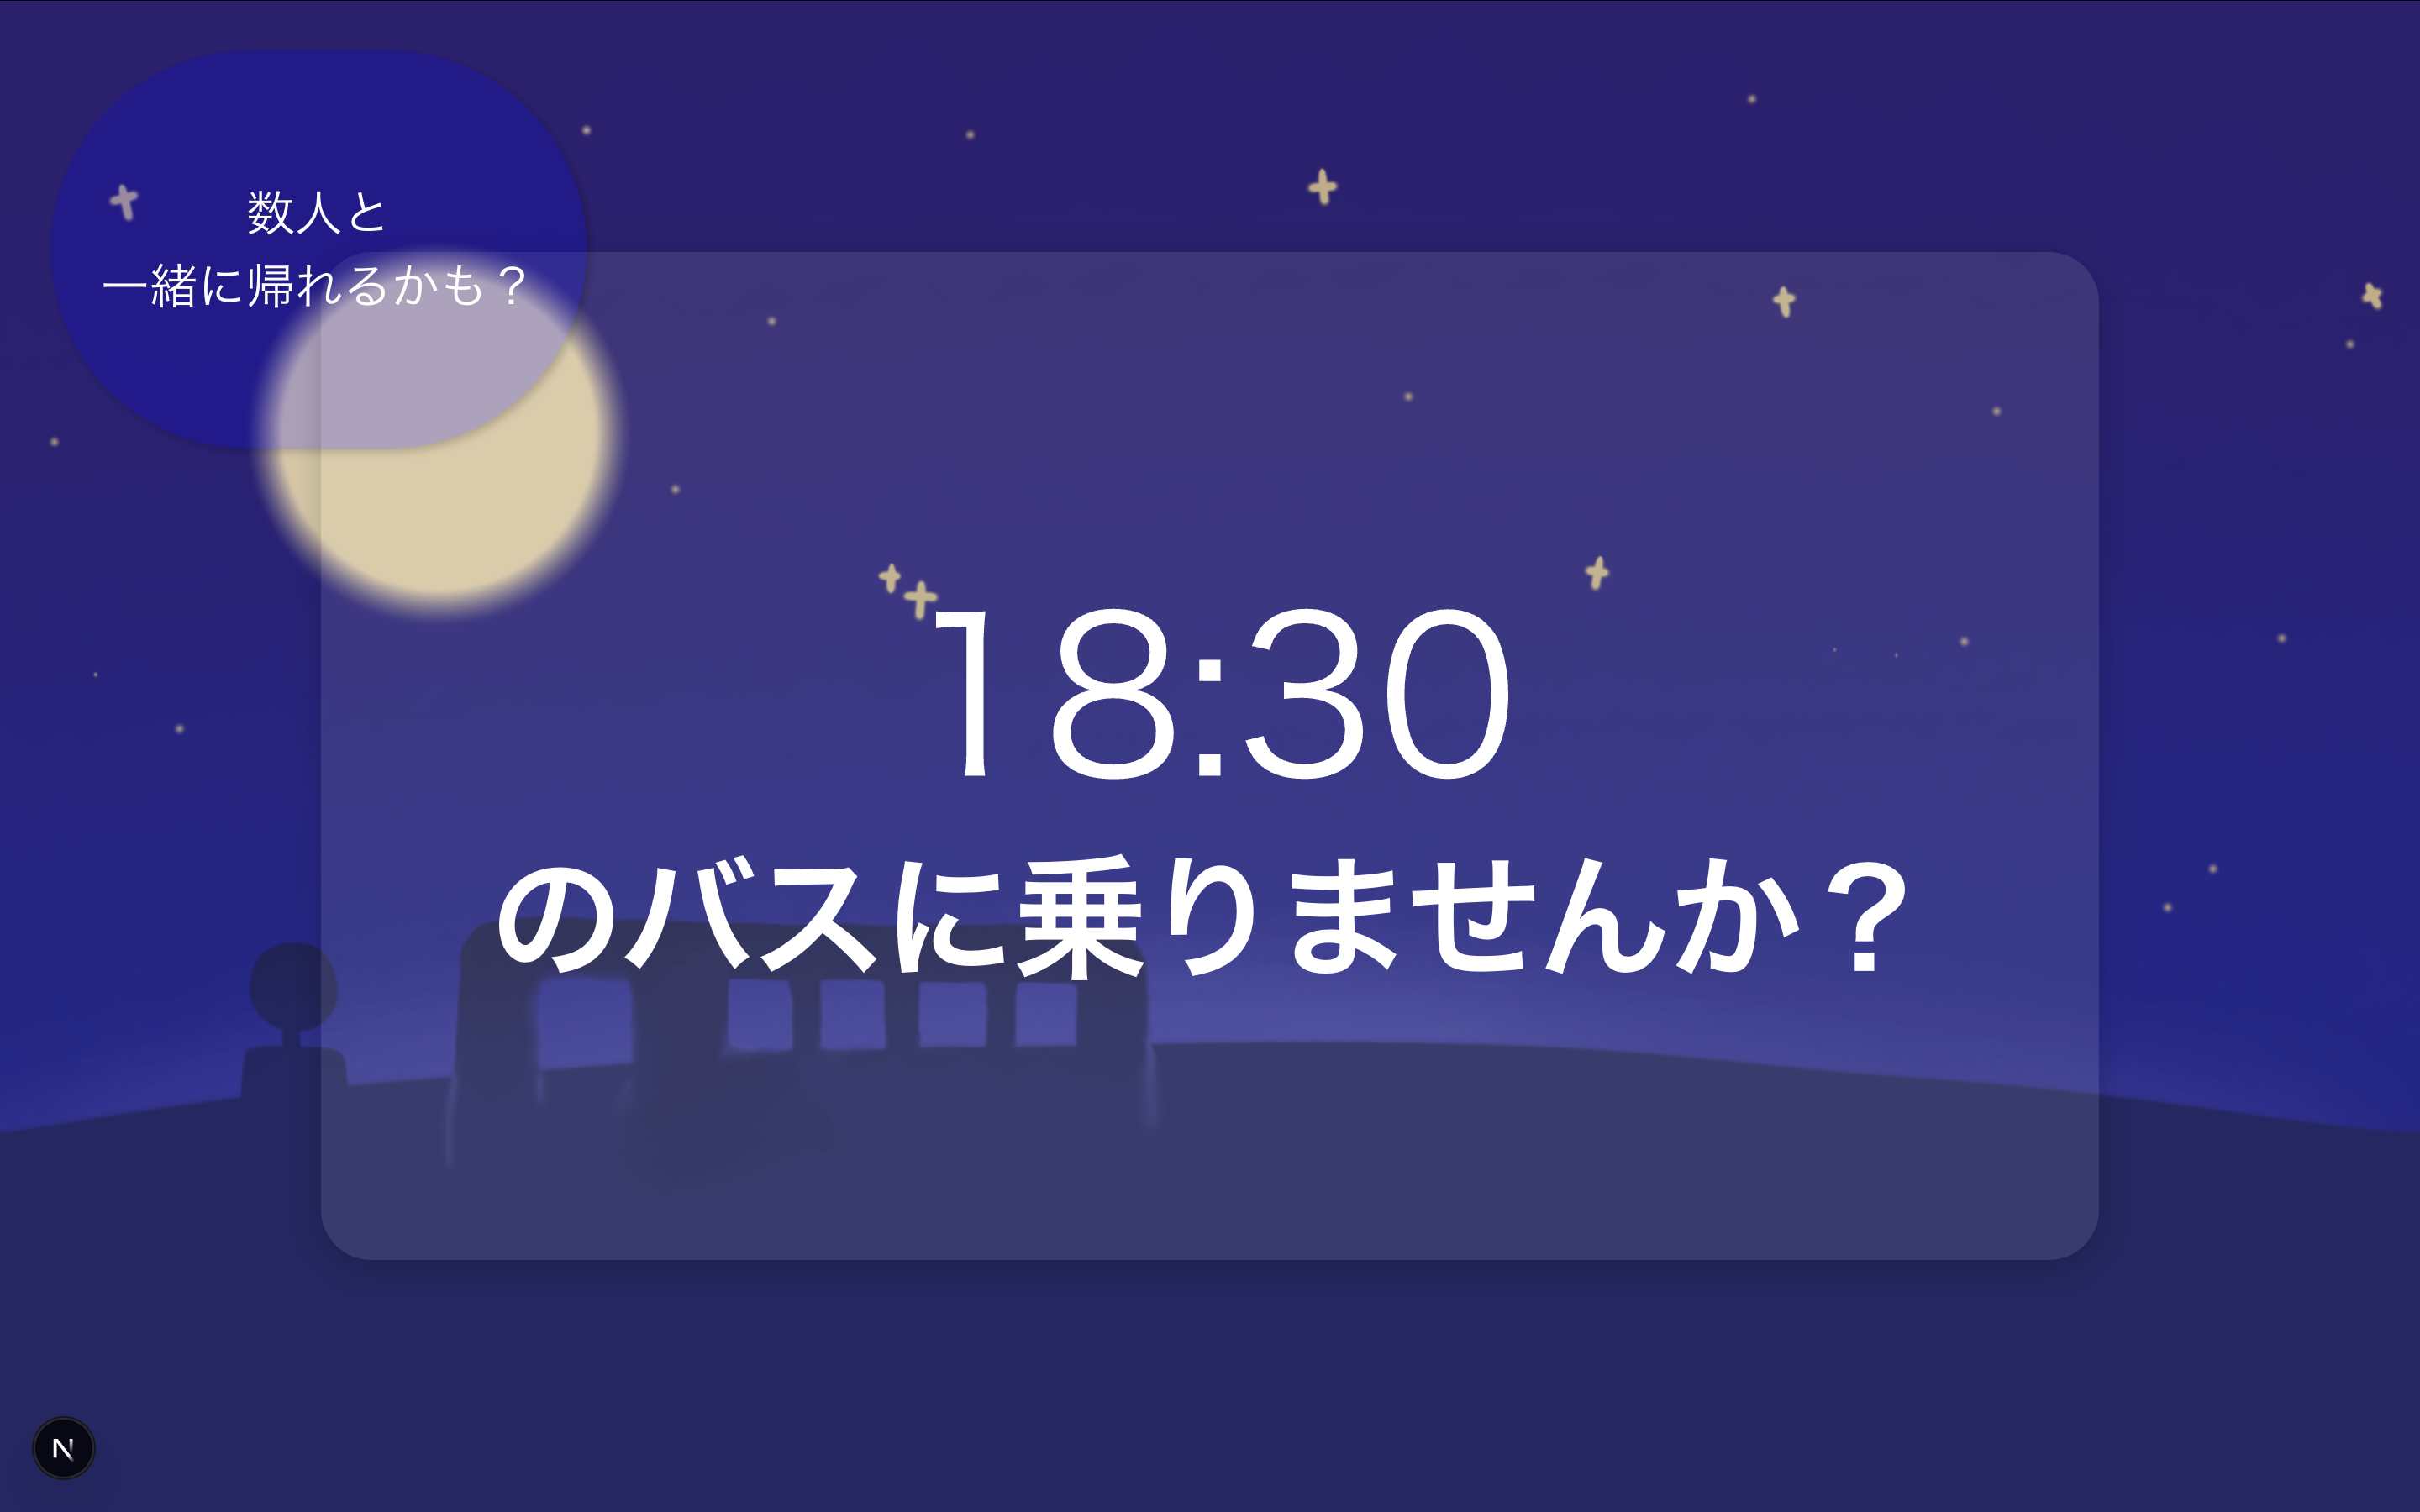
\includegraphics[width=0.7\linewidth]{resultDisplay.png} % suzuki
  \caption{最多投票の時刻を提示する画面}
  \label{fig:resultDisplay}

\end{figure}

% 本画面においても，離れた位置から内容を把握できるよう，帰宅時刻を画面内で大きく表示する設計とした．
% 本画面は，三択の投票結果をもとに，利用者の帰宅行動を一つの時刻へ収束させることを目的としている．
% 投票数が最も多かった時刻を強調して提示し，その時刻に帰宅可能な利用者が比較的多いと視覚的に示す設計とした．
% また，投票がなかった場合には，最も帰りやすいと考えられる帰宅推奨時刻に近い時刻を表示する．
% 同票の時刻が存在する場合には，各時刻の帰宅同行が成立する可能性が同程度であると判断し，より多くの利用者が帰宅行動を起こす前の時刻として，早い時刻を選択する．
% 一方で，投票人数に関する情報は，画面に近づいた際に確認できる程度の大きさとした．
% これにより，帰宅意思を持つ利用者が詳細情報を確認しやすくなる一方で，周囲にいる他の利用者に対して過度な情報提示とならないよう配慮している．
本画面においても，離れた位置から内容を把握できるよう，帰宅時刻を画面内で大きく表示する設計とした．
また，投票数が最も多かった時刻を強調して提示し，三択の投票結果の中で帰宅可能なユーザが比較的多い時刻を視覚的に示す．
一方で，投票人数に関する情報は，画面に近づいた際に確認できる程度の大きさとした．

本画面は，三択の投票結果をもとに，ユーザが帰宅しやすい時刻を一つに絞り込む目的で設計している．
したがって，投票がなかった場合には最も帰宅しやすいと考えられる帰宅推奨時刻に近い時刻を選択する．
同票の時刻が存在する場合には，各時刻の帰宅同行が成立する可能性が同程度であると判断し，より多くのユーザが帰宅行動を起こす前の時刻として，早い時刻を選択する．
また，投票人数の表示方法についても，声かけを行う際の心理的負担を抑える観点から設計している．

なお，本システムでは「おすすめの退室時刻」ではなく，利用者が目標とする行動の基準として「乗車すべきバスの時刻」を提示している．
これは，「この時刻までに出れば余裕をもって間に合う時刻」と「実際に出発すれば間に合う最終的な時刻」との間に存在する時間帯において，何も情報が提示されない状態を避けるためである．
また，この時間帯のみ表示内容や画面構成を切り替えると，利用者にとって表示規則が分かりにくくなる可能性がある．
そのため，本画面では一貫してバスの時刻を基準とした提示に専念し，実際に建物を出る時刻の判断は利用者に委ねる設計とした．


投票人数の表示方法については，人数の多寡によって表現を切り替えている(図\ref{fig:resultDisplays})．
具体的には，無投票の場合は人数表示を行わず，1票の場合には「数人と一緒に帰れるかも？」という抽象的な表現を用いた．
2票以上の場合には「〜人と一緒に帰れるかも？」と具体的な人数を示す．
これは，投票したユーザがその時刻に帰宅可能であると仮定し，「一緒に帰れる可能性」を提示し，声かけを行う際の心理的なハードルを下げる意図で設計した．

\begin{figure}[htb]
  \centering
  \subcaptionbox{無投票の場合}{
    
\includegraphics[width=0.3\linewidth]{0.png}}	% suzuki
  \hspace{3mm}
  \subcaptionbox{投票数が1の場合}{
    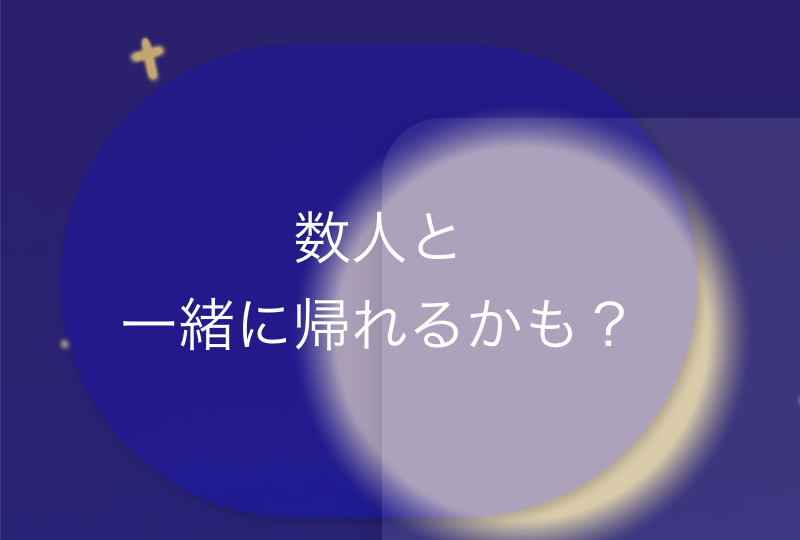
\includegraphics[width=0.3\linewidth]{1.png}}	% suzuki 
  \hspace{3mm}
  \subcaptionbox{投票数が複数の場合}{
    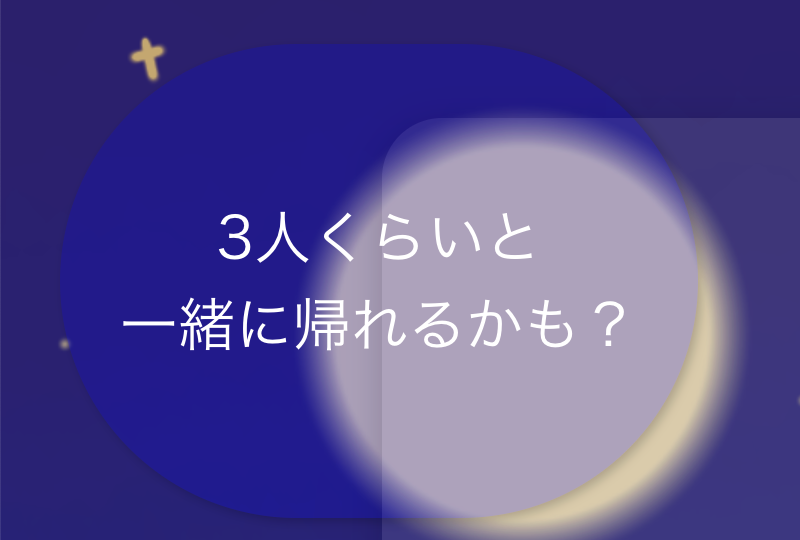
\includegraphics[width=0.3\linewidth]{3.png}}
  \caption{投票人数の提示箇所}
  \label{fig:resultDisplays}
\end{figure}